\section{Examples}

In this section, examples will be given of the libraries described above. The several libraries may be used in each example.

\subsection{Extract Efficiency from Satimo}
In the following example, the efficiency of an antenna is extracted. In order to do this, calibration measurements must be added to the \texttt{calfiles} list. The \texttt{reffiles} list contains reference data of the antennas used for calibration. \emph{Note, that the files from these two lists must be written in ascending order, i.e.\ lowest frequency first}. In this example, the file \texttt{antenna\_meas.trx} is the antenna from which the efficiency is extracted. The output is saved to the file shown in Figure~\ref{fig:pp_example1}.

\lstinputlisting[caption={Extracting efficiency from Satimo.}, label=lst:ex1]{sec/post_processing/examples/example1.py}

\begin{figure}[htbp]
    \centering
    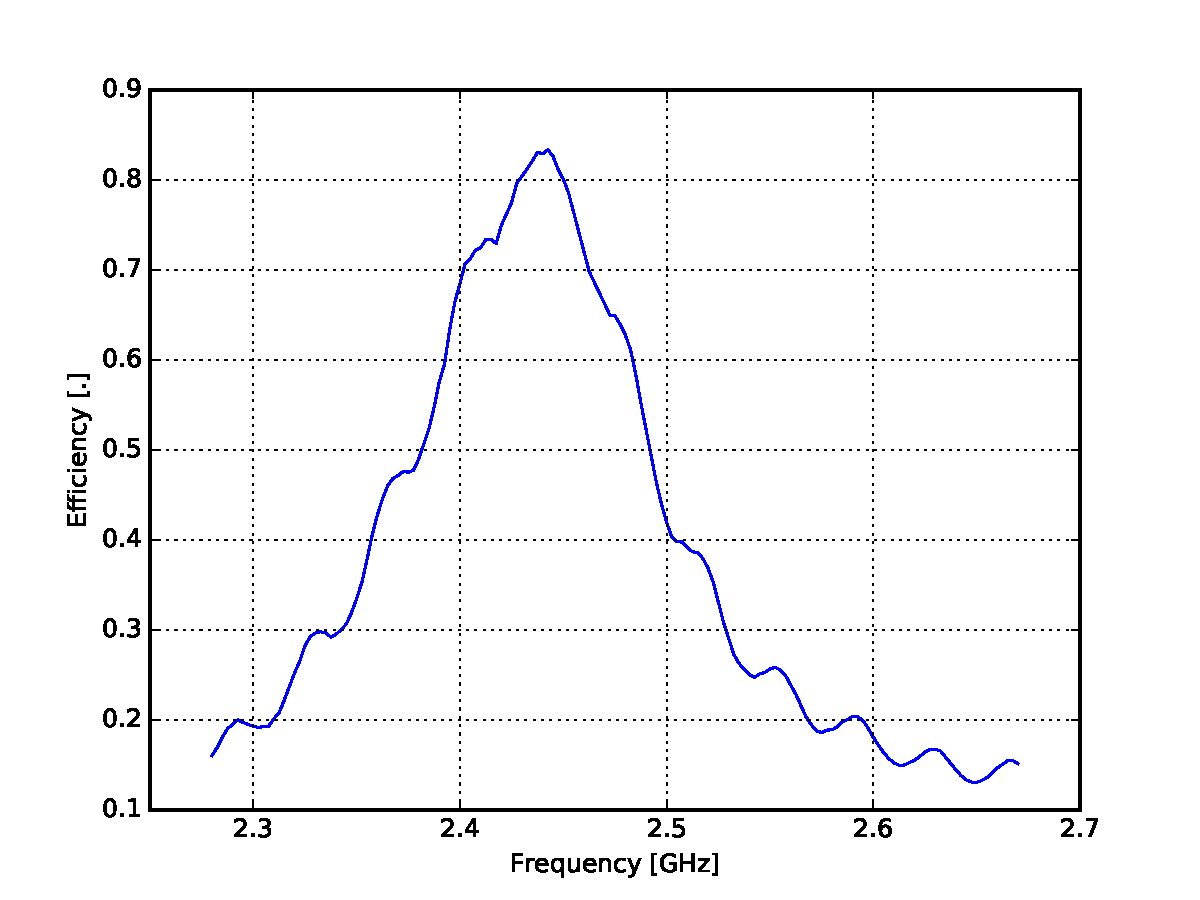
\includegraphics[scale=0.5]{sec/post_processing/examples/ex1_efficiency.pdf}
    \caption{Output from Listing~\ref{lst:ex1}.}
    \label{fig:pp_example1}
\end{figure}


\subsection{Plot 3D Farfield}
The (rough) farfield directly exported from Satimo's 15 probes can be plotted in 3D as shown below. The result is shown in Figure~\ref{fig:pp_example2}. A similar plot -- a 2D color plot -- is also plotted.

\lstinputlisting[caption={Plot 3D Farfield.}, label=lst:ex2]{sec/post_processing/examples/example2.py}

\begin{figure}[htbp]
    \centering
    \begin{subfigure}{0.49\linewidth}
        \centering
        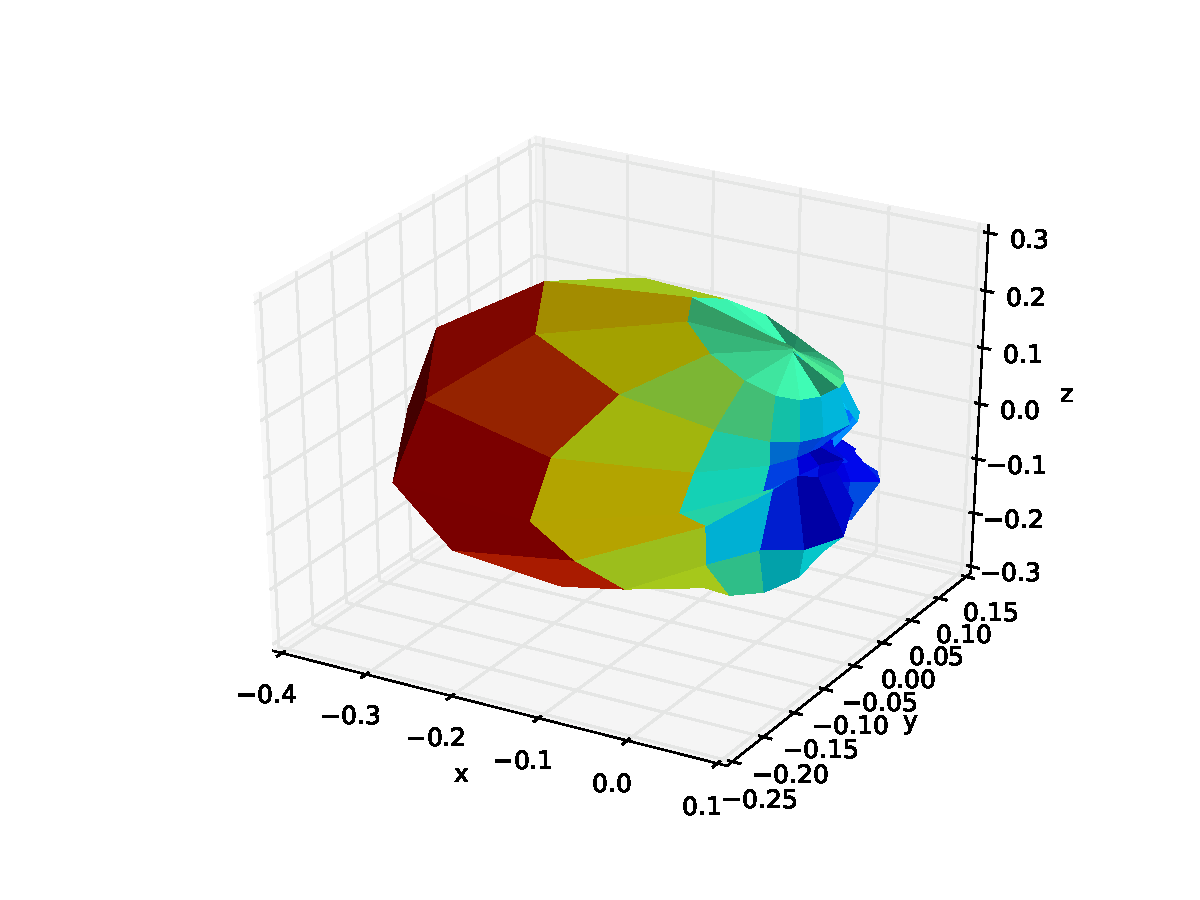
\includegraphics[scale=0.5]{sec/post_processing/examples/ex2_3dfarfield.pdf}
        \caption{3D.}
    \end{subfigure}
    \hfill
    \begin{subfigure}{0.49\linewidth}
        \centering
        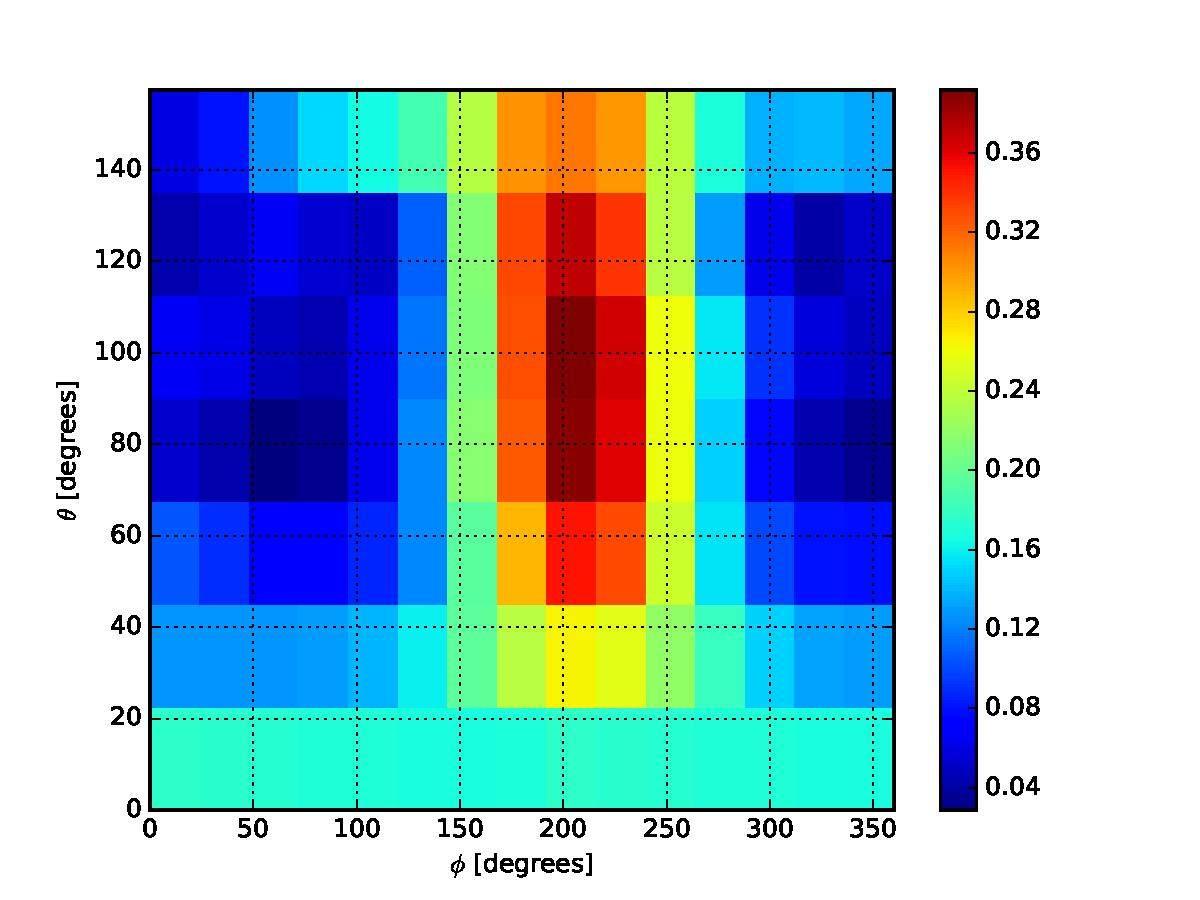
\includegraphics[scale=0.5]{sec/post_processing/examples/ex2_2dfarfield.pdf}
        \caption{2D.}
    \end{subfigure}
    \caption{Output from Listing~\ref{lst:ex2}.}
    \label{fig:pp_example2}
\end{figure}

\subsection{Import a Farfield from CST}
The following example will import and plot a farfield from CST. The farfield should be exported under the Post Processing tab. The output is shown in Figure~\ref{fig:pp_example3}.

\lstinputlisting[caption={Import a Farfield from CST.}, label=lst:ex3]{sec/post_processing/examples/example3.py}


\begin{figure}[htbp]
    \centering
    \begin{subfigure}{0.49\linewidth}
        \centering
        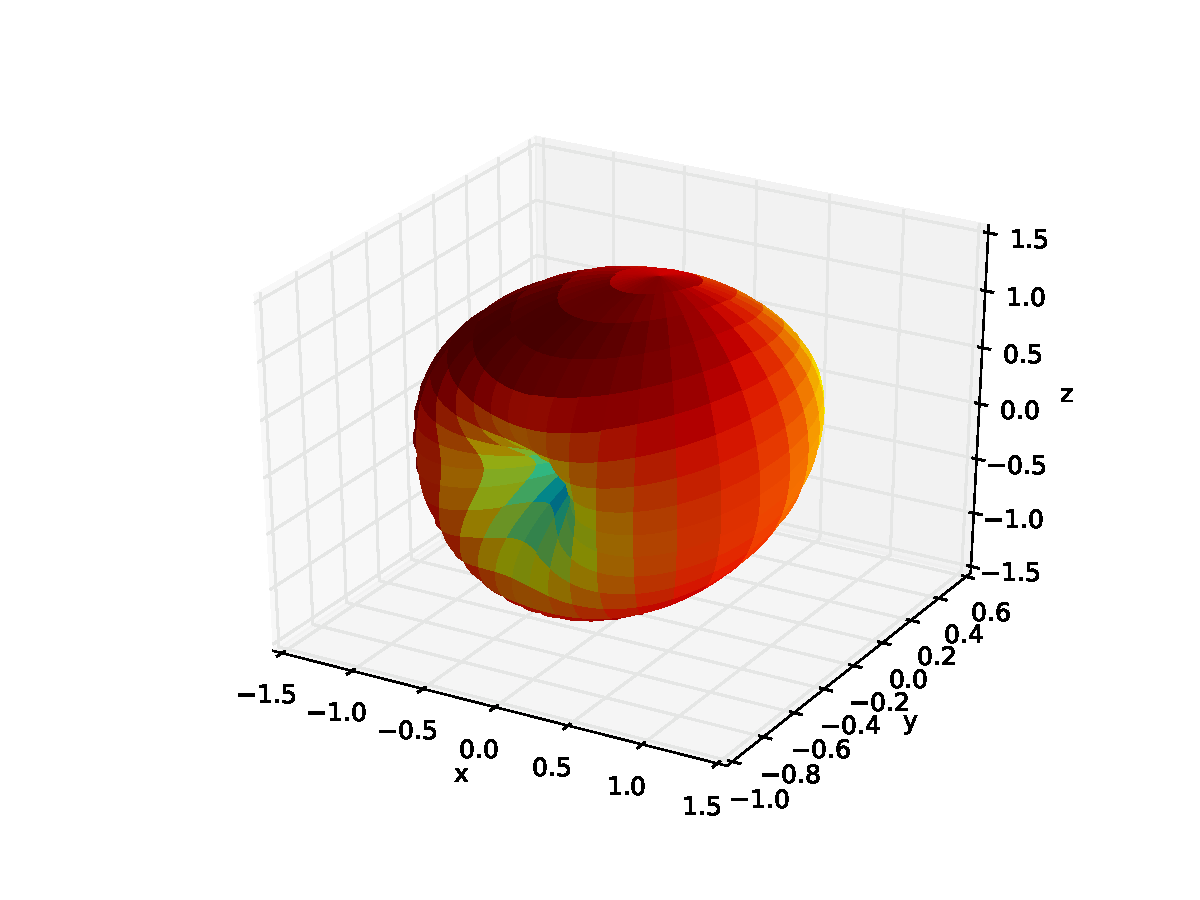
\includegraphics[scale=0.5]{sec/post_processing/examples/ex3_3dfarfield.pdf}
        \caption{3D.}
    \end{subfigure}
    \hfill
    \begin{subfigure}{0.49\linewidth}
        \centering
        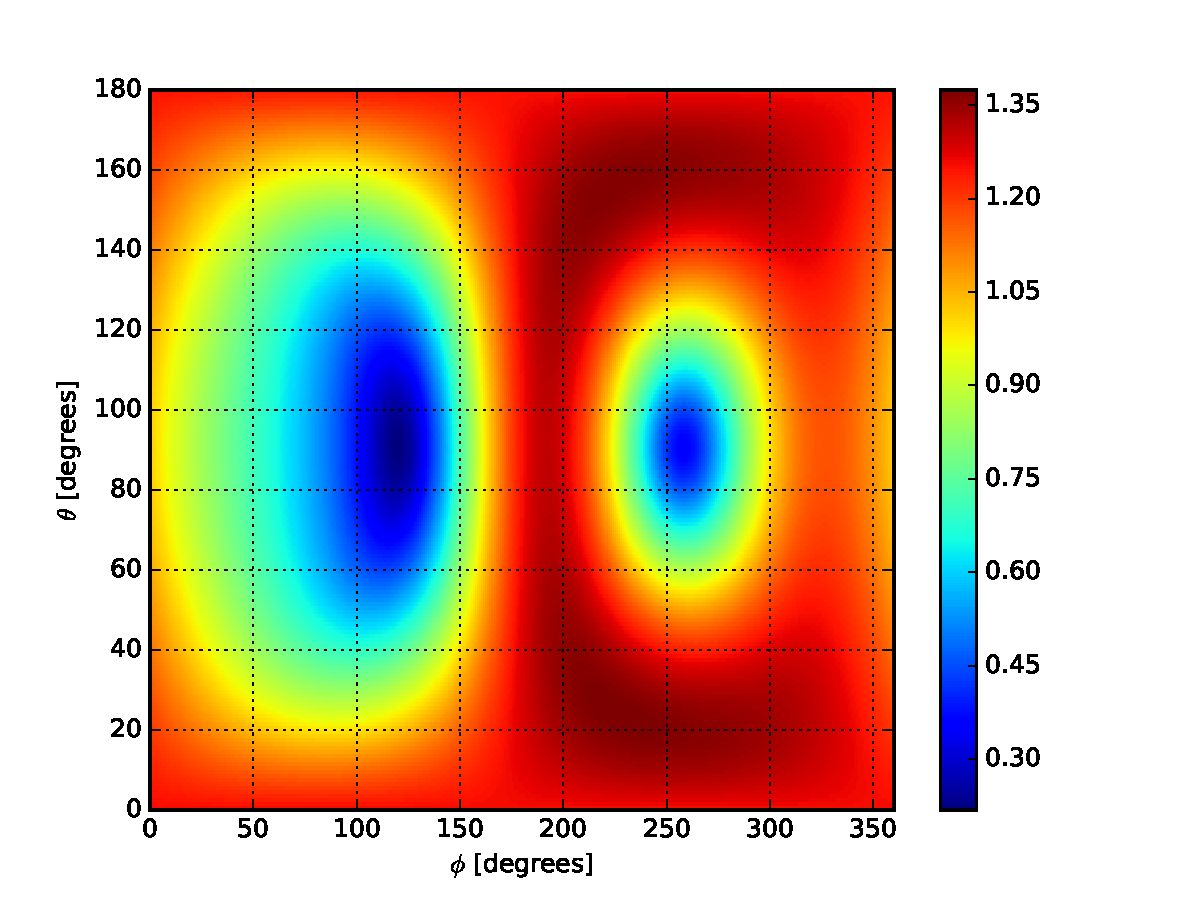
\includegraphics[scale=0.5]{sec/post_processing/examples/ex3_2dfarfield.pdf}
        \caption{2D.}
    \end{subfigure}
    \caption{Output from Listing~\ref{lst:ex3}.}
    \label{fig:pp_example3}
\end{figure}

\subsection{Export Efficiency for Further Analysis}
Using python and numpy, analysis and comparison can be done just as easily as in MATLAB. However, if one is more familiar with MATLAB or need the data for other software, it is advantageous to export the data. Here is a simple example of exporting the efficiency as a data file.

\lstinputlisting[caption={Export efficiency for further analysis.}, label=lst:ex4]{sec/post_processing/examples/example4.py}

The output is a tab-separated file (\texttt{ex4\_efficiency.txt}) which can easily be imported into MATLAB or similar software.

\subsection{Plots for IEEEtran Articles}
It is often desirable to export graphs in a format that is compliant with the text used articles. In the standard IEEEtran format, a \emph{Times} font is used. For figures, the default font size is 8\,pt. The column width is \SI{3.5}{inches}. In the example, the figure size is set to $\SI{3.5}{inches}\times \SI{3}{inches}$.

Note that math symbols can easily be used in figure text (e.g.\ labels) in the same way as symbols are written in \LaTeX, e.g.\ ``\verb|$\theta$ in degrees|'' becomes ``$\theta$ in degrees''.

The result is shown in Figure~\ref{fig:pp_example5}.

\lstinputlisting[caption={Plots for IEEEtran articles.}, label=lst:ex5]{sec/post_processing/examples/example5.py}

\begin{figure}[htbp]
    \centering
    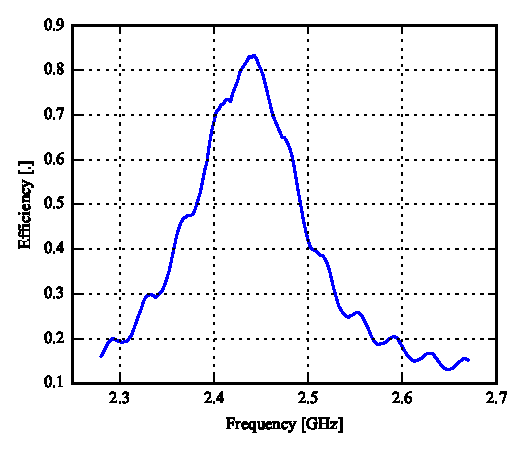
\includegraphics{sec/post_processing/examples/ex5_efficiency.pdf}
    \caption{Output from Listing~\ref{lst:ex5}.}
    \label{fig:pp_example5}
\end{figure}

\subsection{aauplot: Plot S-Parameters}
In the following script, a CSV file from a VNA is plotted using the aauplot library. The output is shown in Figure~\ref{fig:aauplot_ex1}

\lstinputlisting[caption{aauplot: Plot S-parameters}, label=lst:aauplot1]{sec/post_processing/examples_aauplot/ex1.py}

\begin{figure}[htbp]
    \centering
    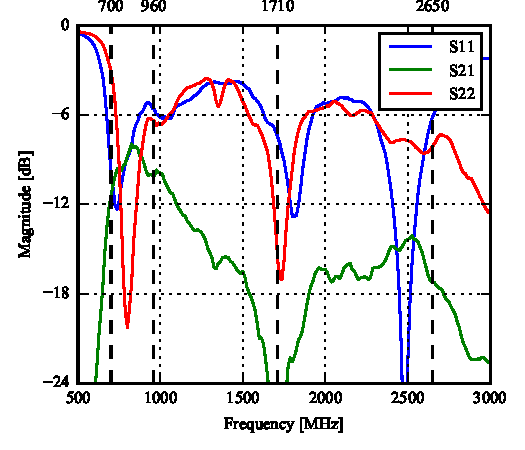
\includegraphics{sec/post_processing/examples_aauplot/ex1_sparams.pdf}
    \caption{Output from Listing~\ref{lst:aauplot1}.}
    \label{fig:aauplot_ex1}
\end{figure}

\subsection{aauplot: Plot Efficiency}
The Satimo library is here used to extract the efficiency of an antenna measured in the Satimo chamber. The aauplot library is used to plot the result. Note that, as opposed to the efficiency example shown above, a calibration table is computed prior to analysis. This means that the calibration is only loaded once, making the processing faster. This can be done when several measurements from the same calibration are analyzed. The result is shown in Figure~\ref{fig:aauplot_ex2}.

\lstinputlisting[caption={aauplot: Plot Efficiency}, label=lst:aauplot2]{sec/post_processing/examples_aauplot/ex2.py}

\begin{figure}[htbp]
    \centering
    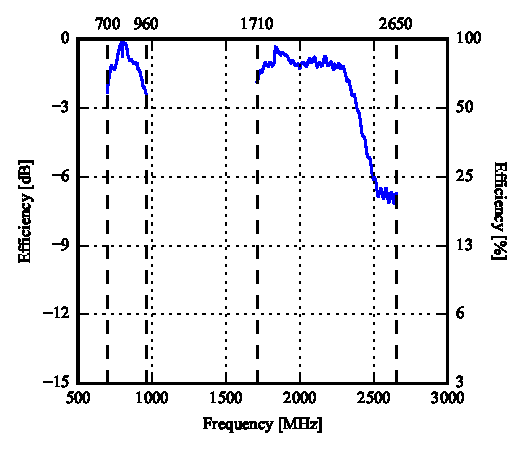
\includegraphics{sec/post_processing/examples_aauplot/ex2_efficiency}
    \caption{Output from Listing~\ref{lst:aauplot2}.}
    \label{fig:aauplot_ex2}
\end{figure}

\subsection{aauplot: Plot Correlation from a Satimo Measurement}
In this example, the farfield of two antennas measured in Satimo. The Satimo Library and the aauplot library is used to plot the envelope correlation coefficient. The result is shown in Figure~\ref{fig:aauplot_ex3}. Note that the two measured antennas must be positioned in \emph{exactly} the same position.

\lstinputlisting[caption={aauplot: Plot correlation from a Satimo measurement.}, label=lst:aauplot3]{sec/post_processing/examples_aauplot/ex3.py}

\begin{figure}[htbp]
    \centering
    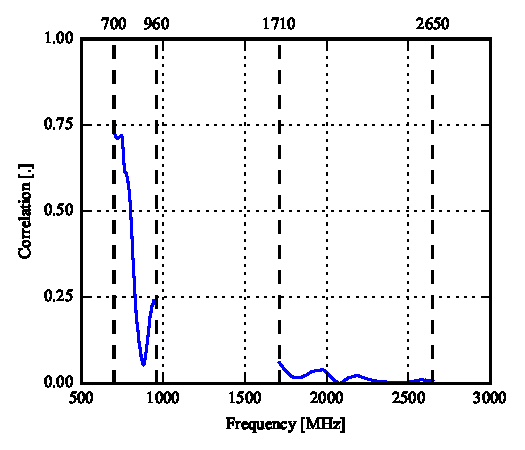
\includegraphics{sec/post_processing/examples_aauplot/ex3_correlation}
    \caption{Output from Listing~\ref{lst:aauplot3}.}
    \label{fig:aauplot_ex3}
\end{figure}

\fixme{Write ``install'' section}
